\documentclass[openany]{book}
\usepackage{ln}

\title{EECS 127 Lecture Notes}
\author{Dun-Ming Huang}
\pgfplotsset{compat=1.18}
\setcounter{chapter}{0}

\begin{document}
\maketitle
\setcounter{tocdepth}{1}
Surprise, there might be weird typos.
These typos are to be revised before exams, and only occassionally after lectures.
\tableofcontents
%\begin{comment}
\chapter{Introduction and Least Squares}
For this lecture, we will traverse through the Spring 2023 versions of course logistics, and then an introduction towards optimization.

\section{An Introductory Prompt}
In this course, we discuss a problem in Computer Science called, ``optimization''.
Understanding optimization is not limited to just understanding mathematical details, and has more to do with ``problem formulation'': for whatever technology comes, optimization is an involved technique of critical thinking.

\section{Administratives, Summary}
\textbf{Logistics.} For Discussion, Homework policies, please check the lecture slides. Friday sections are equivalent to the subsequent Monday sections. \\
\textbf{Advices from Instructor.} Do homeworks, collaborate with people. \\
\textbf{New: Projects.} We will have an option to do a project at the end of the semester, where we complete a project of choice.
This is an effort to bridge the gap between students and research experience; where, provided a research paper, the student will extend that literature at the end of project.
This will count towards grade and remove weight from exams if the project grade helps.
Schemes will be announced. Projects will be in groups, released after the midterm and due during RRR week.

\section{Introduction to The Subject Topic: Optimization}
Optimization is an approach to problems. \\
It is the technique where we attempt to optimize some statistic resembling of a result.
For example, in machine learning from DATA C100 (or EECS 16A/B), we have chosen appropriate loss functions for our learning task to characterize the performance of a model:
\begin{bindenum}
    \item Minimizing the MSE of a linear regresssion model.
    \item Minimizing the cross-entropy loss of a logistic regression model.
    \item Minimizing the distance traveled by an agent in a maze.
\end{bindenum}
Here, we model learning tasks and attempt to optimize a metric. Depending on how we model and represent a problem, the model will perform differently on its learning task.
Therefore, optimization is a study about ``picking the right loss function'' for some same objective.
We consider these design choices, study how they affect learning process.

For another example, Air Traffic control is another optimization problem (at the point of writing, US has just experienced a flight paralysis); for another example, queueing and revenue computation are also common optimization problems.
Optimization itself is omnipresent in modern applications.

In this course, we will learn about:
\begin{bindenum}
    \item Low rank approximation
    \item Ridge regression
    \item Stochastic Gradient Descent
    \item Dual Program (which always provides a lower bound for some optimization problem)
    \item Applications: LQR Control, Classification, SVM
\end{bindenum}

Let's get into the Math now!!!

\subsection{An Example of Problem Formulation}
Say, we work in an oil production firm (I know, very US).
We are allowed to make 10,000 barrels of crude oil, which may be produced into either \textit{Jet Fuel} or \textit{Gasoline}. \\
For every barrel of Jet Fuel produced, a revenue of 30 cents; for Gasoline, 20 cents. Meanwhile, 1 barrel of crude oil produces 0.6 barrels of Jet Fuel or 0.7 barrels of Gasoline. \\
Furthermore, the firm demands that we produce more than some amount of Jet Fuel and Gasoline (respectively, say, 1000 and 2000 barrels). \\
Finally, there are transportation capacities, where 180000 barrel miles are available. Distributing Gasoline costs 30 miles, and distributing Jet Fuel costs 10 miles. \\

We have now been presented a prompt: provided the above conditions, how can I maximize my revenue? \\
Let us first formulate this prompt mathematically:
\[
    \begin{cases}
        x_j = \text{ Quantity of Jet Fuel in barrels} \\
        x_g = \text{ Quantity of Gasoline in barrels}
    \end{cases}
\]
The revenue we generate would be formulated as
\[R(x_j, x_g) = 0.3 x_j + 0.2 x_g\]
such that we are presented the \textbf{constraints}:
\[
    \begin{cases}
        \text{Production Quantity Minimum: } &x_j \geq 1000, x_g \geq 2000 \\
        \text{Total Available Resources: } &\frac{x_j}{0.7} + \frac{x_g}{0.6} \leq 10000 \\
        \text{Transportation Capacity: } &10 x_j + 30 x_g \leq 180000
    \end{cases}
\]
which are mathematically translated from the above English text.

In an optimization framework, we formualte a problem with the following frame:
\begin{ln-explain}{Formulating Optimization Problems}{}
    In a general optimization problem, we attempt to minimize some function $f_0(\vec{x})$, such that some constraint exists:
    \[\forall i \in \{1, \dots, m\}, f_i(\vec{x}) \leq b_i\]
    and here, $\vec{x}$ is listed as a representation of some system's state, existing within the domain of possible inputs (states). \\
    The general objective of optimization is to find a state of system that minimizes $f_0(\vec{x})$, which we mathematically express the solution as:
    \[\vec{x}^* = {argmin}_{\forall i \in \{1, \dots, m\}, f_i(\vec{x}) \leq b_i} f_0(\vec{x})\]
\end{ln-explain}
See the example from above, and try matching the parts of optimization problem with the above framework!

There are some more types of optimization problems! One of them is the famous Least Squares Regression:

\section{Least Squares Regression}
The problem statement:
\begin{center}
    For some matrix $A$ and a vector $\vec{b}$, solve for:
    \[\min_{\vec{x}} {\lvert\lvert A \vec{x} - \vec{b} \rvert\rvert}_2^2\]
\end{center}

Such problem can be widely applied to many mathematical problems, such as regression and projection.

\begin{ln-explain}{Formulating Least Squaresd Regression}{}
    Provided a dataset of points:
    \[\{(x_1, y_1), \dots, (x_n, y_n)\}\]
    where we attempt to model a linear equation
    \[y = mx + c\]
    
    First of all, what is the variable we attempt to search/optimize for? It would be $m, c$ that are the unknowns. \\
    To formulate the Least Squares Problem, we would need to formulate our linear equation for points into some matrix-vector multiplication, and knowing that we are solving for $m$ and $c$, the formulation follows:
    \[
        A
        \begin{bmatrix} m \\ c \end{bmatrix}
        = \vec{b}
    \]
    Let us now fill in the contents of $A$ and $\vec{b}$ for formulation, where $A$ and $\vec{b}$ are of known quantities:
    \[
        \begin{bmatrix} \vec{x} & \vec{1} \end{bmatrix}
        \begin{bmatrix} m \\ c \end{bmatrix}
        = \vec{y}
    \]
\end{ln-explain}
From prior coursework we also know that there is a closed-form solution:
\[\vec{x}^* = {(A^T A)}^{-1} A^T \vec{b}\]
for matrices $A$ with nontrivial nullspaces (see EECS16A for a proof that $N(A) = N(A^T A)$).

\begin{ln-explain}{Closed-Form Solution of Least Squares}{}
    To minimize the L2 norm of difference between $A \vec{x}$ and $\vec{b}$, we attempt to find a vector $\vec{x}$ that minimizes the differences between them. \\
    Note that for any choice of $\vec{x}$, it is by definition that $A \vec{x} \in Col(A)$. \\

    We now face two claims that we resolve to proceed on solving this problem:
    \begin{bindenum}
        \item[1.] The endpoint of ${proj}_{Col(A)} \vec{b}$ is the point closest to the endpoint of $\vec{b}$ (if they share a same starting point) in $Col(A)$.
        \item[2.] $\vec{OP} = A \vec{x}^*$, where $\vec{x}^*$ has the closed-form solution as previously described.
    \end{bindenum}

    Claim 1 can be proven by contradiction: assume another point $C$ closer than $P$ to $B$ (such that $\vec{OB}$ is closer to $\vec{b}$). However, Pythagorean Theorem argues against it. \\
    Claim 2 is a series of algebraic manipulation as outlined in previous courseworks, based on that the error vector $\vec{e} = \vec{b} - A\vec{x}$ should be orthogonal to the columnspace $Col(A)$ by geometry:
    \begin{align*}
        A^T \vec{e} &= 0 \\
        A^T (A \vec{x}^* - \vec{b}) &= 0 \\
        A^T A \vec{x}^* &= A^T \vec{b} \\
        \vec{x}^* &= {(A^T A)}^{-1} A^T \vec{b}
    \end{align*}
    Such result is also known as the \textbf{Normal Equation}.
\end{ln-explain}

Interestingly, Least Squares Algorithm has a quadratic property, causing it to be some parabolic object that performs a \textbf{convex function} to optimize along; that is, the local minimum of this function is a global minimum.

\newpage
\chapter{
    Linear Algebra Bootcamp: Norms, Gram-Schmidt, QR, FTLA
}

\section{Vectors and Norms}
In the previous lecture, we have recognized the following symbol:
\begin{ln-symbol}{Euclidean Norm}{}
    The Euclidiean Norm, otherwise known as a \textbf{2-Norm}, is a mathematical quantity for some vector $\vec{x}$:
    \[
        {\lVert \vec{x} \rVert}_2 = \sqrt{\sum_i x_i^2}
    \]
    which measures the distance between the starting and terminal point of a vector.
\end{ln-symbol}
However, there exist more norms to that. Particularly, \textbf{norms} are functions that satisfy the following properties:
\begin{ln-define}{Norm}{}
    A norm is a function $f: \mathcal{X} \rightarrow \R$ such that:
    \begin{bindenum}
        \item[1.] Non-negativeness: $\forall \vec{x} \in \mathcal{X}, \lVert \vec{x} \rVert \geq 0$, and $\lVert \vec{x} \rVert = 0 \iff \vec{x} = \vec{0}$
        \item[2.] Triangle Inequality: $\forall \vec{x}, \vec{y} \in \mathcal{X}, \lVert \vec{x} + \vec{y} \rVert \leq \lVert \vec{x} \rVert + \lVert \vec{y} \rVert$
        \item[3.] Scalar Multiplication: $\forall \alpha \in \R, \vec{x} \in \mathcal{X}, \lVert \alpha \vec{x} \rVert = \alpha \lVert \vec{x} \rVert$
    \end{bindenum}
\end{ln-define}
For example, a general family of norms that satisfy the above properties would be the \textbf{LP-norms}:
\begin{ln-define}{LP-Norms}{}
    LP-Norms are norm functions defined as:
    \[
        {\lVert \vec{x} \rVert}_p = {\bigg( \sum_{i = 1}^n |x_i|^p \bigg)}^{\frac{1}{p}}
    \]
    for some natural number $p$. \\
    Particularly, the Euclidean Norm, otherwise known as the \textit{2-norm} is LP-norm with $p = 2$. \\
    And, the interesting observation is:
    \begin{align*}
        {\lVert \vec{x} \rVert}_1 &= \sum_{i = 1}^n |x_i| \\
        {\lVert \vec{x} \rVert}_\infty &= \max_{i = 1, \dots, n} |x_i| \\
    \end{align*}
\end{ln-define}

\section{Cauchy-Schwartz Inequality}
This inequality was active in EECS 16A!
\begin{ln-define}{Cauchy-Schwartz Inequality}{}
    The inequality is phrased as:
    \[
        |\vec{x}^T \vec{y}| \leq {\lVert \vec{x} \rVert}_2 {\lVert \vec{y} \rVert}_2
    \]
    And using the property,
    \[|\forall x \in \R, |\cos(x)| \leq 1\]
    this inequality originates from the following algebraic work:
    \begin{align*}
        |\langle \vec{x}, \vec{y} \rangle| &= |\vec{x}^T \vec{y}| = |\vec{y}^T \vec{x}| \\
        &= |{\lVert \vec{x} \rVert}_2 {\lVert \vec{y} \rVert}_2 \cos(\theta_{\vec{x}, \vec{y}})| \\
        &\leq |{\lVert \vec{x} \rVert}_2 {\lVert \vec{y} \rVert}_2|
    \end{align*}
\end{ln-define}

The last two lines of the above derivation is justified by the mechanics along which we find the projection of $\vec{x}$ onto $\vec{y}$:
\[
    {proj}_{\vec{x}}^{\vec{y}} = \vec{y} \frac{\vec{x}^T\vec{y}}{{\lVert \vec{y} \rVert}_2^2}
\]
Where, since the projection is a multiple of $\vec{y}$ such that ${proj}_{\vec{x}}^{\vec{y}} = t\vec{y}$, we also recognize that,
\[
    \cos(\theta_{\vec{x}, \vec{y}}) = \frac{{\lVert t\vec{y} \rVert}_2}{{\lVert \vec{x} \rVert}_2}
\]
And upon matching the two equations, I acquire:
\begin{align*}
    t = \cos(\theta_{\vec{x}, \vec{y}}) \frac{{\lVert t\vec{x} \rVert}_2}{{\lVert \vec{y} \rVert}_2} &= \frac{\vec{x}^T\vec{y}}{{\lVert \vec{y} \rVert}_2^2} \\
    |{\lVert \vec{x} \rVert}_2 {\lVert \vec{y} \rVert}_2| &= \langle \vec{x}, \vec{y} \rangle
\end{align*}

\subsection{Holder's Inequality and Norm Ball}
In fact, we find that the Cauchy-Schwartz is a general case of this inequality:
\begin{ln-define}{Holder's Inequality}{}
    Provided the quantities
    \[\vec{x}, \vec{y} \in \R^n, \text{and some } p, q \geq 1 \text{ s.t. } \frac{1}{p} + \frac{1}{q} = 1\]
    Then, 
    \[|\vec{x}^T \vec{y}| \leq {\lVert \vec{x} \rVert}_p{\lVert \vec{y} \rVert}_p\]
\end{ln-define}
From this concept, let us consider the concept of \textit{``norm ball''}: the geographical object containing all vectors such that their lp-norm is $1$.

\begin{bindenum}
    \item For a $2-norm$, for example, the norm ball looks like a unit circle (containing all 2D vectors with length $1$, hence a circle of radius $1$).
    \item For a $1-norm$, similar logic guides us to a diagonally placed circle (rotated $45^\circ$) centered at the origin with side lengths $2$.
    \item For the $\infty-norm$, has a norm ball of a square centered at origin with side length $2$. This embeds the unit ball from $2-norm$, which embeds the unit ball from $1-norm$.
\end{bindenum}
In this sense, the area of norm ball is larger for any increase in $p$ such that it embeds the prior norm balls.

\begin{ln-explain}{Optimization Problem Regarding Norm Ball}{}
    \textbf{Problem Formulation:} Solve for \[\max_{{\Vert \vec{x} \rVert}_2 \leq 1} \vec{x}^T \vec{y}\]
    \tcblower
    \textbf{p = 2}: The solution would be, by the Cauchy Schwartz's implication,
    \[\vec{x}^* = \frac{\vec{y}}{\lVert \vec{y} \rVert}_2\]
    \textbf{p = 1}: The expression of dot product is equivalently
    \[x_1 y_1 + \cdots + x_n y_n\]
    Where the constraint is
    \[|x_1| + \cdots + |x_n| \leq 1\]
    For each value the components of $\vec{x}$, which is finite and upper bounded by $1$, we should allocate maximum contribution to the maximum element of $\vec{y}$ to maximize this dot product (a weighted sum of $\vec{y}$'s component, essentially). \\
    Therefore, let $i$ be the index at which $\vec{y}$ has the component of largest absolute value,
    \begin{quote}
        There is an achievable solution for $\vec{x}^*$, being the unit vector $\vec{e}_i$ multiplied by $sgn(y_i)$, so to counter for cases where $\vec{y}$ is negative.
    \end{quote}
    \par
    In turn, we see that
    \[\vec{x}^T \vec{y} = \max_i |y_i| = {\lVert \vec{y} \rVert}_\infty\]
    Meanwhile, let us use the Holder's Inequality to achieve a more rigorous proof. Holder's Inequality states that,
    \[
        |\vec{x}^T \vec{y}| \leq {\lVert \vec{x} \rVert}_1 {\lVert \vec{y} \rVert}_\infty = \max_i |y_i|
    \]
    Where,
    \begin{quote}
        \textbf{The formulation in above section shows achievability, and Holder's Inequality expresses an upper bound to prove the approach correct.}
    \end{quote}
    \textbf{\textit{Alternative proof of p = 1 via Triangle Inequality}}: Via the triangle inequality, we acquire:
    \begin{align*}
        |\vec{x}^T \vec{y}| &= |\sum_i x_i y_i| \\
        &\underset{Triangle\ Inequality}{\leq} \sum_i |x_i y_i| \\
        &= \sum_i |x_i||y_i| \\
        &\leq \sum_i |x_i| \max_i |y_i| = \max_i |y_i| = {\lVert \vec{x} \rVert}_\infty
    \end{align*}
    We see that the upperbound of $|\vec{x}^T \vec{y}|$ \textbf{has an upperbound} that is \textbf{achievable}, assembling all necessary aspects of a complete proof. \\
    \textbf{p = $\infty$}: We can find upper bound via Holder's Inequality,
    \[
        |\vec{x}^T \vec{y}| \leq {\lVert \vec{x} \rVert}_1 {\lVert \vec{y} \rVert}_\infty = \sum_i |y_i|
    \]
    The infinity norm of $\vec{x}$ shows the constraint that:
    \[
        \max_i |x_i| = 1
    \]
    and we may simply compute:
    \[
        x_i = sgn(y_i)
    \]
    to find and certify the achievability of this upper bound.
\end{ln-explain}

\section{Gram-Schmidt Orthonormalization and QR Decomposition}
Gram-Schmidt Orthonormalization is an algorithmic technique to find an orthonormal basis for a set of vectors. \\
The procedure of such algorithm is portrayed as defined in the following cell:
\begin{ln-define}{The Procedure of Gram-Schmidt Orthonormalization}{}
    Let us have a set of vectors $\{\vec{a_1}, \dots, \vec{a_n}\}$.
    \begin{bindenum}
        \item[1] $\vec{q_1} = \frac{\vec{a_1}}{{\lVert \vec{a_1} \rVert}_2}$
        \item[2] for $i$ in $\{2, \dots, n\}$:
        \item[3] \hspace{0.6cm} $\vec{z_i} = {proj}_{\{\vec{q_1}, \dots, \vec{q_{i - 1}}\}} \vec{a_i}$
        \item[4] \hspace{0.6cm} $\vec{s_i} = \vec{a_i} - \vec{z_i}$
        \item[5] \hspace{0.6cm} $\vec{q_i} = \frac{\vec{s_i}}{{\lVert \vec{s_i} \rVert}_2}$
        \item[6] return $\{\vec{q_1}, \dots, \vec{q_n}\}$
    \end{bindenum}
    And note that,
    \[
        \vec{z_i} = \sum_{j = 1}^{i - 1} \vec{q_j} \langle \vec{a_i}, \vec{q_j} \rangle
    \]
\end{ln-define}

\newpage
\chapter{Linear Algebra: Symmetric Matrices}

\section{Fundamental Theorem of Linear Algebra}
\begin{ln-theorem}{Orthogonal Decomposition of Space}{}
    Let us consider some vector space $\mathcal{X}$ and some subspace $\mathcal{S} \subseteq \mathcal{X}$. \\
    Then, we may state that,
    \[\forall \vec{x} \in \mathcal{X}, \vec{x} = \vec{s} + \vec{r} \text{ uniquely, s.t. } \vec{s} \in \mathcal{S} \land \vec{r} \in \mathcal{S}^\perp\]
    such that, 
    \[\mathcal{S}^\perp = \{\vec{y} : \langle \vec{x}, \vec{y} \rangle = 0, \vec{x} \in \mathcal{S}\}\]
    Conseuqeuntially, we are stating that for the space $\mathcal{X}$,
    \[\mathcal{X} = \mathcal{S} \oplus \mathcal{S}^\perp\]
    it is a \textbf{direct sum} of the vector spaces $\mathcal{S}$ and $\mathcal{S}^\perp$ (we may write any vector in $\mathcal{X}$ as the sum of two components where each component belongs to some specific subspace of the direct sum.)
\end{ln-theorem}
This leads to a theorem about decomposing a vector space from some given matrix:
\begin{ln-theorem}{Fundamental Theorem of Linear Algebra}{}
    \textbf{Theorem.} Consider a matrix $A \in \R^{m \times n}$, then,
    \[\R^n = N(A) \oplus R(A^T)\]
    where, similarly,
    \[\R^m = \mathcal{R}(A) \oplus N(A^T)\]
    \tcblower
    \textbf{Proof.} We may use Orthogonal Decomposition of Space (Theorem 3.1.1) to aid our proof. If so, we would only need to show the two following facts:
    \begin{enumerate}
        \item $N(A) \perp \mathcal{R}(A^T)$, or equivalently, $N(A) = \mathcal{R}(A^T)^\perp$
        \item $N(A^T) \perp \mathcal{R}(A)$
    \end{enumerate}
    Let us perform a proof on the first fact, which would be to prove the equivalence of two sets. \\
    First, we may prove that $N(A) \subseteq \mathcal{R}(A^T)^\perp$:
    \begin{quote}
        Suppose that there is an arbitrary vector $\vec{u} \in N(A)$, where $A \vec{u} = \vec{0}$. \\
        Then, we realize that,
        \[(A \vec{u}) = \vec{0}, \vec{0}^T = \vec{u}^T A^T\]
        then, for any arbitrary vector $\vec{u}'$, we may find that
        \[\vec{u}^T A^T \vec{u}' = \vec{0}^T \vec{u}' = 0\]
        Therefore, the vector $\vec{u}$ is orthogonal to any vector belonging to $\mathcal{R}(A^T)$, which would mathematically state,
        \[\vec{u} \in \mathcal{R}(A^T)^\perp\]
    \end{quote}
    Then, we may prove the opposite direction: $\mathcal{R}(A^T)^\perp \subseteq N(A)$
    \begin{quote}
        Suppose that there is an arbitrary vector $\vec{w} \in \mathcal{R}(A^T)$, and $\vec{x} \in \mathcal{R}(A^T)^\perp$; by which, we would state for the arbitrary pair $(\vec{w}, \vec{x})$ that
        \[
            \forall \vec{w} \in \mathcal{R}(A^T), \vec{x} \in \vec{x} \mathcal{R}(A^T)^\perp (\vec{x} \cdot \vec{w} = 0)
        \]
        Thus, $\forall \vec{w} \in \mathcal{R}(A^T)$:
        \begin{align*}
            \langle \vec{x}, \vec{w} \rangle &= 0 \\
            \langle \vec{x}, A^T \vec{w} \rangle &= 0 \\
            \vec{x}^T A^T \vec{w} &= 0
        \end{align*}
        Which qualifies us to state that $A \vec{x} = \vec{0}$. \\
        Therefore, $\vec{x} \in N(A)$.
    \end{quote}
    Applying a symmetrical proof to the second fact allows us to provide a complete proof for this theorem.
\end{ln-theorem}

\section{Minimum Norm Problem}
This is some sister problem to the Least Squares Problem:
\begin{center}
    \begin{tabular}{l || l}
        Least Squares & Minimum Norm \\
        \hline
        \hline
        Solves an overdetermined system & Solves an underdetermined system \\
        \hline
        Formulation: $\min_{\vec{x}} {\lVert A\vec{x} - \vec{b} \rVert}_2^2$ & Formulation: $\min_{A\vec{x} = \vec{b}} {\lVert \vec{x} \rVert}_2^2$
    \end{tabular}
\end{center}
\begin{ln-explain}{Solution to Minimum Norm Problem}{}
    Let us provide some $\vec{x}$ that is a solution to $A \vec{x} = \vec{b} \neq \vec{0}$. \\
    Some component of $\vec{x}$ might belong to the nullspace of $A$. Meanwhile, we also acknowledge that $\vec{x}$ is some arbitrary vector in the real space.
    Therefore, the vector $\vec{x}$ may be decomposed into $\vec{x} = \vec{n} + \vec{r}$, where 
    \[
        \vec{n} \in N(A), \vec{r} \in \mathcal{R}(A^T)
    \]
    In that case, we now minimize for $\vec{r} \in \mathcal{R}(A^T)$ under the setup that,
    \[
        A \vec{x} = A(\vec{n} + \vec{r}) = A \vec{r} = \vec{b}
    \]
    We may recognize that $\vec{n} \cdot \vec{r} = 0$ due to the orthogonal decomposition's nature. Therefore,
    \[
        {\lVert \vec{x} \rVert}_2^2 = {\lVert \vec{n} \rVert}_2^2 + {\lVert \vec{r} \rVert}_2^2
    \]
    Therefore, $\vec{x}^* = A^T \vec{w}$
    \begin{align*}
        A \vec{x} &= \vec{b} \\
        (A A^T) \vec{w} &= \vec{b} \\
        \vec{w} &= {(A A^T)}^{-1} \vec{b} \\
        \vec{x}^* &= A^T {(A A^T)}^{-1} \vec{b}
    \end{align*}
\end{ln-explain}

\section{Principal Component Analysis}
Principal Component Analysis is a technique to reduce dimensionality in high-dimension datapoints, so to find underlying feature patterns and enable plotting. \\
This can be achieved via projecting data onto a lower dimension structure to recover lower dimensional structure from the original high dimensional data. \\
Mathematically, it would be to project $\vec{x_1}, \dots, \vec{x_n}$ onto $\vec{w} \in \R^p$ such that the projected vectors are all as close to the original vectors as possible.
\begin{ln-explain}{Projections}{}
    For projecting some vector $\vec{x}$ onto $\vec{w}$, we would obtain result
    \[
        {(\vec{w}^T \vec{w})}^{-1} \vec{w}^T \vec{x}
    \]
    Where, projection vector $\vec{x}$ onto a columnspace of matrix $A$ then follows the least squares formula,
    \[
        {(A^T A)}^{-1} A^T \vec{x}
    \]
\end{ln-explain}
Now, let's discuss how would PCA work:
\begin{ln-explain}{PCA as an Optimization Problem}{}
    \textbf{Formulation.} 
    Let the individual projection errors be phrased as
    \[{\lVert \vec{x_i} - \langle \vec{w}, \vec{x_i} \rangle \vec{w} \rVert}_2^2\]
    Where, the average projection error can thus be quantified as,
    \[
        R(\vec{w}) = \frac{1}{n} \sum_{i = 1}^n {\lVert \vec{x_i} - \langle \vec{w}, \vec{x_i} \rangle \vec{w} \rVert}_2^2 = MSE(\vec{w})
    \]
    Therefore, the formulation of optimization problem is:
    \[
        \min_{\vec{w}} R(\vec{w}) \text{ subject to } {\lVert \vec{w} \rVert}_2^2 = 1
    \]
    And the assumption of PCA dataset is that it is zero-meaned, because de-meaned data will allow less bias when deciding the weight vector for PCA.
    \tcblower
    \textbf{Solution.}
    Let us consider the projection error,
    \[
        {\lVert \vec{x_i} - \langle \vec{w}, \vec{x_i} \rangle \vec{w} \rVert}_2^2 = {\lVert \vec{e_i} \rVert}_2^2
    \]
    The error can be algebraically simplified:
    \begin{align*}
        {\lVert \vec{e_i} \rVert}_2^2
        &= {(\vec{x_i} - \langle \vec{w}, \vec{x_i} \rangle \vec{w})}^T \cdot (\vec{x_i} - \langle \vec{w}, \vec{x_i} \rangle \vec{w}) \\
        &= {\lVert \vec{x_i} \rVert}_2^2 - 2 {\langle \vec{x_i}, \vec{w} \rangle}^2 + {\langle \vec{x_i}, \vec{w} \rangle}^2 {\lVert \vec{w_i} \rVert}_2^2 \\
        &= {\lVert \vec{x_i} \rVert}_2^2 - {\langle \vec{x_i}, \vec{w} \rangle}^2
    \end{align*}
    Therefore, removing the fixed costs in the error, we are essentially facing the following optimization problem:
    \[
        \max_{\vec{w}} \frac{1}{n} \sum_{i = 1}^n {\langle \vec{x_i}, \vec{w} \rangle}^2
    \]
\end{ln-explain}

\newpage
\chapter{Principal Component Analysis}

\section{Symmetric Matrix}
Let us begin with a formal definition of Symmetric Matrix:
\begin{ln-define}{Symmetric Matrix}{}
    A matrix $A \in \R^{n \times n}$ is a \textbf{symmetric matrix} if
    \[A = A^T\]
    or equivalently,
    \[\forall i, j \in \{1, \cdots, n\}, a_{i,j} = a_{j,i}\]
    and in such case we express,
    \[A \in \mathbb{S}^n\]
\end{ln-define}
Symmetric Matrices have such properties summarized by the Spectral Theorem:
\begin{ln-theorem}{Spectral Theorem}{}
    If $A \in \mathbb{S}^n$, then:
    \begin{bindenum}
        \item[1.] All of its eigenvalues are real.
        \item[2.] Eigenspaces corresponding to distinct eigenvalues are orthogonal.
        \item[3.] The algebraic multiplicity of an eigenvalue is equal to its geometric multiplicity
        \subitem (alternatively, the matrix is diagonalizable, such that there exists an orthonormal $U$ and diagonal $\Sigma$ to compose $A = U \Sigma U^T$).
    \end{bindenum}
    An interlude here:
    \begin{ln-define}{Multiplicity of Eigenvalues}{}
        A review from EECS 16B:
        \begin{bindenum}
            \item The algebraic multiplicity of an eigenvalue $(m_A)$ is the number of times such eigenvalue appears in its matrix's characteristic polynomial.
            \item The geometric multiplicity of an eigenvalue $(m_G)$ is the number of lienarly independent eigenvectors that such eigenvalue corresponds to.
        \end{bindenum}
    \end{ln-define}
\end{ln-theorem}
Meanwhile, symmetric matrices also enjoy special properties in their eigenvalues:
\begin{ln-theorem}{Variational Characteristics of Rayleigh Coefficient}{}
    The Rayleigh Coefficient of some symmetric matrix $A \in \mathcal{S}^n$ and vector $\vec{x} \in \R^n$ is defined as:
    \[
        R_{A, \vec{x}} = \frac{\vec{x}^T A \vec{x}}{\vec{x}^T \vec{x}}
    \]
    \textbf{Theorem.}
    Then, we may acknowledge via proof that:
    \[
        \forall \vec{x} \neq \vec{0}, \lambda_{min}(A) \leq R_{A, \vec{x}} \leq \lambda_{max}(A)
    \]
    and alternatively we may formulate the above inequality such that,
    \[
        \begin{cases}
            \lambda_{max}(A) = \max_{{\lVert \vec{x} \rVert}_2^2 = 1}\vec{x}^T A \vec{x} \\
            \lambda_{min}(A) = \min_{{\lVert \vec{x} \rVert}_2^2 = 1}\vec{x}^T A \vec{x}
        \end{cases}
    \]
    \tcblower
    \textbf{Proof.}
    Let us define that $\vec{y} = U^T \vec{x}$, and we will proceed onto the algebraic work:
    \begin{align*}
        \vec{x}^T A \vec{x}
        &= \vec{x} U \Lambda U^T \vec{x} \\
        &= \vec{y}^T \Lambda \vec{y} \\
        {\lVert \vec{y} \rVert}_2^2 &= 1
    \end{align*}
    And, furthermore,
    \begin{align*}
        \vec{y}^T \Lambda \vec{y}
        &= \sum \lambda_i y_i^2 \\
        &< \sum \lambda_{max} y_i^2 = \lambda_{max} \\
        \vec{y}^T \Lambda \vec{y}
        &= \sum \lambda_i y_i^2 \\
        &> \sum \lambda_{min} y_i^2 = \lambda_{min}
    \end{align*}
    So we have now found the upper bound and lower bound of the optimization problem, justifying the boundaries of inequality. \\
    And, we may also acknowledge that providing $\vec{x}$ as the normalized eigenvector of maximum and minimum eigenvalues provide the solution for achieving the lower and upper bound:
    \begin{align*}
        \vec{v}_{\lambda_{max}}^T A \vec{v}_{\lambda_{max}}
        &= \lambda_{max} {\lVert \vec{v}_{\lambda_{max}} \rVert}_2^2 \\
        &= \lambda_{max} \\
        \vec{v}_{\lambda_{min}}^T A \vec{v}_{\lambda_{min}}
        &= \lambda_{min} {\lVert \vec{v}_{\lambda_{min}} \rVert}_2^2 \\
        &= \lambda_{min}
    \end{align*}
\end{ln-theorem}
Below, let us discuss how we may use the properties of symmetric matrices to solve Principal Component Analysis, which is a problem we were studying in the previous lecture.

\section{PCA}
\begin{quote}
    Principal Component Analysis is a technique to reduce dimensionality in high-dimension datapoints, so to find underlying feature patterns and enable plotting.
    This can be achieved via projecting data onto a lower dimension structure to recover lower dimensional structure from the original high dimensional data. \\
\end{quote}
We will pick up from last lecture with a new formulation for optimization problem:
\begin{ln-explain}{Introduction of Principal Component Analysis as Problem}{}
    Suppose we have a set of vectors:
    \[
        \{\vec{x_1}, \dots, \vec{x_n}\}, \forall i (\vec{v_i} \in \R^p)
    \]
    And we would like to project our data into a lower dimensional subspace, such that we may reduce computational cost, and projected vectors are close to the original data.
\end{ln-explain}
Let us find the first principal component, $\vec{w}$, then, such that the dataset projected on this direction is as close to the original data as possible. Then, we will repeat the process of:
\begin{bindenum}
    \item Find principal component $\vec{w_i}$
    \item[$\downarrow$] Remove all projected components onto principal component $i$
    \item Repeat process to find principal component $\vec{w_{i + 1}}$
\end{bindenum}
Let us now formulate the mathematical aspects of PCA:
\begin{ln-explain}{Mathematical Formulation of Principal Component Analysis as Problem}{}
    \textbf{Metric of Optimization.}
    Suppose we have a set of vectors:
    \[
        \{\vec{x_1}, \dots, \vec{x_n}\}, \forall i (\vec{v_i} \in \R^p)
    \]
    Let us find a vector $\vec{w}$ such that:
    \[
        \begin{cases}
            {\lVert \vec{w} \rVert}_2 = 1 \\
            MSE(\vec{w}) = \frac{1}{n} \sum_{i = 1}^n e_i^2
        \end{cases}
    \]
    where, the individual error terms were defined and derived into:
    \begin{align*}
        {\lVert \vec{e_i} \rVert}_2^2
        &= {(\vec{x_i} - \langle \vec{w}, \vec{x_i} \rangle \vec{w})}^T \cdot (\vec{x_i} - \langle \vec{w}, \vec{x_i} \rangle \vec{w}) \\
        &= {\lVert \vec{x_i} \rVert}_2^2 - 2 {\langle \vec{x_i}, \vec{w} \rangle}^2 + {\langle \vec{x_i}, \vec{w} \rangle}^2 {\lVert \vec{w_i} \rVert}_2^2 \\
        &= {\lVert \vec{x_i} \rVert}_2^2 - {\langle \vec{x_i}, \vec{w} \rangle}^2
    \end{align*}
    Therefore,
    \[
        MSE(\vec{w}) = \frac{1}{n} \sum_{i = 1}^n ({\lVert \vec{x} \rVert}_2^2 - {\langle \vec{w}, \vec{x_i} \rangle}^2)
    \]
    \tcblower
    \textbf{Formulation of Optimization.}
    To consider the optimization problem holistically, we should formulate that,
    \[
        \underset{\vec{w}}{argmin} MSE(\vec{w}) = \underset{\vec{w}}{argmin} -\frac{1}{n} \sum_{i = 1}^n {\langle \vec{w}, \vec{x_i} \rangle}^2
    \]
    which is equivalently solving for
    \[
        \underset{\vec{w}}{argmax} \frac{1}{n} \sum_{i = 1}^n {\langle \vec{w}, \vec{x_i} \rangle}^2
    \]
    and we would recognize so becuase the aspect of MSE, $\frac{1}{n} \sum_{i = 1}^n {\lVert \vec{x} \rVert}_2^2$, is a fixed cost.
\end{ln-explain}
Now, let us attempt to solve for the above formulation:
\begin{ln-explain}{Solving PCA Optimization Problem}{}
    Keep in mind that our data matrix would appear as:
    \[
        X = \begin{bmatrix} \vec{x_1}^T \\ \vdots \\ \vec{x_n}^T \end{bmatrix}
    \]
    We may begin with the algebraic work then.
    \[
        X \vec{w} = \begin{bmatrix} \vec{x_1}^T \vec{w} \\ \vdots \\ \vec{x_n}^T \vec{w} \end{bmatrix}
    \]
    Let us capture the information and make some algebraic derivation:
    \begin{align*}
        \frac{1}{n} \sum {\langle \vec{w}, \vec{x_i} \rangle}^2
        &= \frac{1}{n} \sum {(\vec{x_i}^T \vec{w})}^2 \\
        &= \frac{1}{n} {\lVert X \vec{w} \rVert}_2^2 \\
        &= \vec{w}^T \frac{X^T X}{n} \vec{w}
    \end{align*}
    We call the matrix in above intermediate form the covariance matrix:
    \[
        C = \frac{X^T X}{n} = C^T
    \]
    And, using the knowledge from Section 4.1, we obtain that the solution of:
    \[
        {argmax}_{\vec{w}} \vec{w}^T C \vec{w} \text{ subject to } {\lVert \vec{w} \rVert}_2^2
    \]
    would be the eigenvector of $\lambda_{max}(C)$.
\end{ln-explain}

\newpage
\chapter{SVD and Low-Rank Approximation}

\section{Singular Value Decomposition (SVD)}
Let us suppose that there is a matrix $A \in \R^{m \times n}$ whose rank is $rk(A) = r$, then there exists a decomposition of $A$ in the shape of:
\[
    A = \sum_{i = 1}^n \sigma_i \vec{u_i} \vec{v_i}^T
\]
where,
\begin{bindenum}
    \item The set $\{\vec{u_1}, \dots, \vec{u_n}\}$ is orthonormal
    \item The set $\{\vec{v_1}, \dots, \vec{v_n}\}$ is orthonormal
    \item $\forall i \in [1, r], \sigma_i > 0$
    \subitem $\forall i \in [1, n], \sigma_i \geq 0$
\end{bindenum}
\begin{ln-symbol}{Compact SVD}{}
    The above dyadic decomposition of SVD written in terms of matrix transformation would be:
    \begin{align*}
        A &=
        \begin{bmatrix} \vec{u_1} & \cdots & \vec{u_r} \end{bmatrix}
        \begin{bmatrix}
            \sigma_1 & & \\
            & \ddots & \\
            & & \sigma_r
        \end{bmatrix}
        \begin{bmatrix} \vec{v_1}^T \\ \vdots \\ \vec{v_r}^T \end{bmatrix} \\
        &= U_r \Sigma_r V_r^T
    \end{align*}
\end{ln-symbol}
Meanwhile, the full SVD that still considers zero-valued $\sigma_i$ is written as follows:
\begin{ln-symbol}{Full SVD}{}
    The formulation follows:
    \begin{align*}
        A &=
        \begin{bmatrix} \vec{u_1} & \cdots & \vec{u_m} \end{bmatrix}
        \begin{bmatrix}
            \Sigma_r & 0 \\
            0 & 0
        \end{bmatrix}
        \begin{bmatrix} \vec{v_1}^T \\ \vdots \\ \vec{v_n}^T \end{bmatrix} \\
        &= U \Sigma V^T
    \end{align*}
    from which, we may observe that the shape of $\Sigma$ is highly dependent on the shape of $A$:
    \begin{bindenum}
        \item If $A$ is tall, so is $\Sigma$
        \item If $A$ is wide, so is $\Sigma$
    \end{bindenum}
\end{ln-symbol}
The squareness of $U$ and $V$ in full SVD allows us to also decompose $A^T A$ as:
\[
    A^T A = {(U \Sigma V^T)}^T (U \Sigma V^T) = V \Sigma^T U^T U \Sigma V^T = V \Sigma^2 V^T
\]
which is more convenient than the compact form SVD that instead uses rectangular $U$ and $V$.

\subsection{Formation of SVD}
As singular vectors are eigenvectors of symmetric matrices $A^T A$, by applying Spectral Theorem, we find that singular vectors of $A$ would all be orthonormal.
Then, let's use this point as an opportunity to praise $A^T A$'s symmetricness:
\begin{ln-theorem}{The Properties and Formation of SVD}{}
    Let the nonzero eigenvalues of $A^T A$ be
    \[
        \lambda_1 \geq \cdots \geq \lambda_r > 0
    \]
    where, upon dimming that $rk(A^T A) = r$, we may obtain $rk(A) = rk(A^T A) = r$ (using rank-nullity theorem, and the fact that $N(A^T A) = N(A)$). \\
    Let us also suppose that orthonormal vectors in $V$ form eigenpairs with the above eigenvalues:
    \[
        \forall i \in [1, r], A^T A \vec{v_i} = \lambda_i \vec{v_i}
    \]
    Now, define that,
    \[
        \sigma_i := \sqrt{\lambda_i}
    \]
    such that:
    \[
        \vec{u_i} := \frac{A \vec{v_i}}{\sigma_i}
    \]
\end{ln-theorem}
Let us now check, whether the above formation grants an orthonormal $U$:
\begin{ln-explain}{Orthonormality of Set of $\vec{u_i}$}{}
    Let us follow the definition of $\vec{u_i}$ from the last block. \\
    Then,
    \[A \vec{v_i} = \sigma_i \vec{u_i}\]
    Suppose now we have some vectors $\vec{u_i}$ and $\vec{u_j}$, then
    \begin{align*}
        \vec{u_i} \cdot \vec{u_j}
        &= \frac{\vec{v_i}^T A^T}{\sigma_i} \frac{A \vec{v_j}}{\sigma_j} \\
        &= \frac{\vec{v_i}^T \lambda_j \vec{v_j}}{\sigma_i \sigma_j} = 0
    \end{align*}
\end{ln-explain}
Now that we have proven the orthonormality and note the definitions of $\vec{u_i}$ and $\vec{v_i}$, we arrive at the conclusion:
\[
    A V = U \Sigma, A = U \Sigma V^T
\]
such arithmetic operation is only possible under the full SVD form (such that $V$ can be noted as orthonormal at all).
This is once again a demonstration of significance of full SVD.

\subsection{Geometry of SVD}
\begin{ln-fig}{Geometric Property of SVD as Transformation}{}
    We may see from the below image's operations,
    \begin{center}
        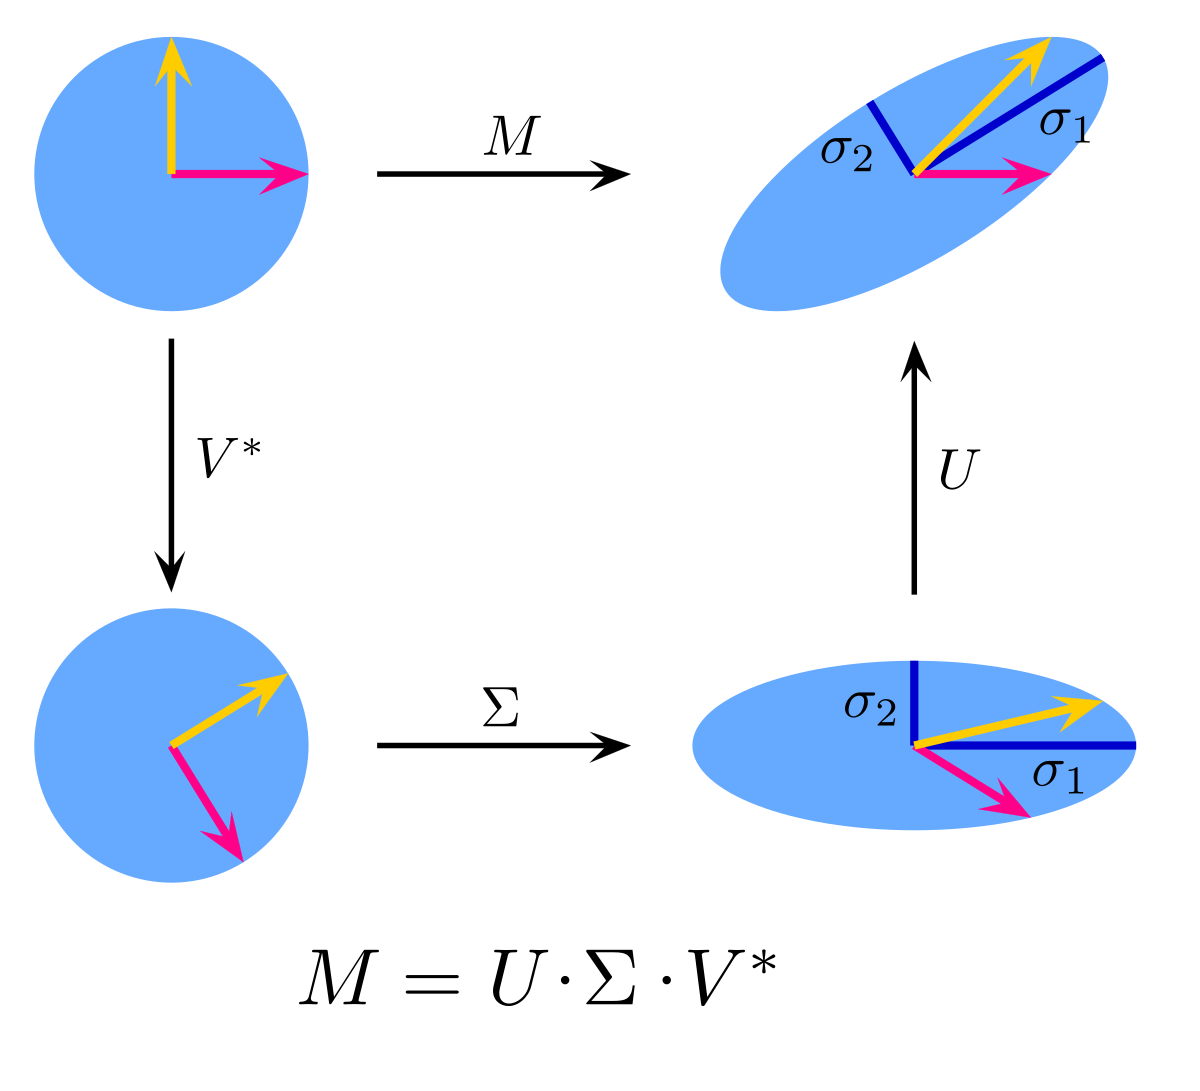
\includegraphics[scale=0.1]{figs/ln05/svd_geometry.png}
    \end{center}
    that SVD is, as priorly mentioned, a combination of three transformations. Where,
    \begin{bindenum}
        \item The orthonormal matrices $U$, $V$ are reflections or rotations.
        \item The matrix $\Sigma$ is a dilation.
    \end{bindenum}
    Furthermore, let us observe the vectors drawn on the unit circle. \\
    Since $V$ is orthonormal, we may conclude that $\vec{v_1} \perp \vec{v_2}$. However, bizzarely, we may also find that
    \[A \vec{v_1} \perp A \vec{v_2}\]
\end{ln-fig}

\section{Low Rank Approximation}
Low Rank Approximation is the task of approximating a matrix $A$ in a lower rank than $rk(A)$, to conserve computational cost and perform efficient computations.

\subsection{Matrix Norms}
Let us first discuss the optimization function of this task: matrix norm.

The norm of matrix also comes in diverse form, because matrices can be interpreted in many forms. \\
For example:
\begin{bindenum}
    \item Chunk of data (like an array)
    \item Operator of transformation
\end{bindenum}
Therefore, along these interpretations, we may present respective definitions of matrix norms.
\begin{ln-define}{Frobenius Norm}{}
    \textit{insert most recent COMPSCI 189 weeder homework PTSD.} \\
    The Frobenius Norm is defined as:
    \[
        \pnorm{A}{F} = \sqrt{\sum_{i = 1}^m \sum_{j = 1}^n A_{i,j}^2} = \sqrt{Trace(A^T A)}
    \]
    This is because the Frobenius inner product may be defined as:
    \[
        {\langle A, B \rangle}_F = Trace(A^T B) = \sum_{i = 1}^n \vec{A_i} \cdot \vec{B_i}
    \]
    and, as we recognize the relation between norm and inner product,
    \[
        \pnorm{A}{F} = \sqrt{{\langle A, A \rangle}_F} = \sqrt{\sum_{i = 1}^n \vec{A_i} \cdot \vec{A_i}}
    \]
\end{ln-define}
The Frobenius Norm has some interesting properties:
\begin{ln-theorem}{Orthonormal Matrices and Frobenius Norm}{}
    Let $U_1 \in \R^{m \times m}$, $A \in \R^{m \times n}$, and $U_2 \in \R^{n \times n}$, where $U_1, U_2$ are orthonormal. \\
    Then,
    \begin{align*}
        \pnorm{U_1 A}{F}
        &= \sqrt{Trace(A^T U_1^T U_1 A)} \\
        &= \sqrt{Trace(A^T A)} = \pnorm{A}{F} \\
        \pnorm{A U_2}{F}
        &= \sqrt{Trace(U_2^T A^T A U_2)} \\
        &\underset{\text{Commutivity in Trace}}{=} \sqrt{Trace(A^T A)} = \pnorm{A}{F} \\
    \end{align*}
\end{ln-theorem}
Now, let's discuss another definition of matrix norm:
\begin{ln-define}{Operator Norm (aka. Spectral Norm, L2-Norm)}{}
    Such norm is defined as:
    \[
        \pnorm{A}{2} = \max_{\pnorm{\vec{x}}{2} = 1} \pnorm{A \vec{x}}{2} = \sigma_{max}(A)
    \]
    \tcblower
    \textbf{Solution to Above Optimization Problem.}
    \begin{align*}
        \max_{\pnorm{\vec{x}}{2} = 1} \pnorm{A \vec{x}}{2}
        = \max_{\pnorm{\vec{x}}{2} = 1} \sqrt{\vec{x}^T A^T A \vec{x}}
        = \sqrt{\lambda_{max}(A^T A)} = \sigma_{max}(A)
    \end{align*}
    Suppose we attach another orthonormal matrix $U$ to the original matrix $A$, then the optimization problem develops a solution fairly similaly:
    \begin{align*}
        \max_{\pnorm{\vec{x}}{2} = 1} \pnorm{AU \vec{x}}{2}
        &= \max_{\pnorm{\vec{x}}{2} = 1} \sqrt{\vec{x}^T U^T A^T A U \vec{x}} \\
        &= \max_{\pnorm{\vec{x}}{2} = 1} \sqrt{\vec{y}^T A^T A \vec{y}} \\
        &= \sqrt{\lambda_{max}(A^T A)} = \sigma_{max}(A)
    \end{align*}
    where since we still find that $\vec{y}$ is normal, the attachment of $U$ providing no change to the optimization problem. \\
    Meanwhile, we find this phenomenon to persist even if $U$ is multiplied from an opposite direction:
    \begin{align*}
        \max_{\pnorm{\vec{x}}{2} = 1} \pnorm{UA \vec{x}}{2}
        &= \max_{\pnorm{\vec{x}}{2} = 1} \sqrt{\vec{x}^T A^T U^T U A \vec{x}} \\
        &= \max_{\pnorm{\vec{x}}{2} = 1} \sqrt{\vec{x}^T A^T A \vec{x}} \\
        &= \sqrt{\lambda_{max}(A^T A)} = \sigma_{max}(A)
    \end{align*}
    Therefore, we may also observe similar properties in norms, where:
    \[
        \pnorm{A}{2} = \pnorm{U_1A}{2} = \pnorm{AU_2}{2} \text{ for orthonormal matrices } U_1, U_2
    \]
\end{ln-define}


\newpage
\chapter{Low-Rank Approximation}

\section{Discussion of L-RA}
Suppose we have some matrix $A \in \R^{m \times n}$, where storing this matrix would take significant computational resources.
Is there a method to store an approximation of this matrix, such that the approximation is more efficient to store for, and we would thus reduce computational cost of storage? \\
We have discussed the possibility of such technique within the previous lecture, where we have solved the optimization problem:
\[\max_{\pnorm{\vec{x}}{2} = 1} \pnorm{A \vec{x}}{2}\]

Today, we will discuss the extension of such solution: Low-Rank Approximation. \\
It would be characterized from the optimization problem:
\[
    \underset{B \in \R^{m \times n}, rk(B) = k}{\text{argmin}} \pnorm{A - B}{F}
\]
where we may see a contextually similar optimization problem:
\[
    \underset{B \in \R^{m \times n}, rk(B) = k}{\text{argmin}} \pnorm{A - B}{2}
\]
Let us perform a proof on this:
\begin{ln-explain}{The LRA Optimization Problem on Spectral Norm}{}
    \textbf{Problem.}
    \[
        \underset{B \in \R^{m \times n}, rk(B) = k}{\text{argmin}} \pnorm{A - B}{2}
    \]
    \tcblower
    \textbf{Solution.} \\
    Keep in mind that our proof proceeds in the direction of:
    \begin{bindenum}
        \item Finding a possible upper bound
        \item Finding the achievability of such upper bound
        \item Finding the legitimacy of such upper bound
    \end{bindenum}
    Now, let us move on with the subparts of a proof. \\
    \par
    \textbf{\textit{Finding a Possible Upper Bound.}} \\
    Let us define
    \[
        A_k = \sum_{i = 1}^k \sigma_i \vec{u_i} \vec{v_i}^T
    \]
    Then, the difference between such approximation and $A$ would be:
    \[\pnorm{A - A_k}{2} = \pnorm{A_n - A_k}{2} = {\Bigg\| \sum_{i = k + 1}^n \sigma_i \vec{u_i} \vec{v_i}^T \Bigg\|}_2\]
    which, following along the optimization problem phrased last lecture, we would obtain the solution to be:
    \[
        {\Bigg\| \sum_{i = k + 1}^n \sigma_i \vec{u_i} \vec{v_i}^T \Bigg\|}_2 = \sigma_{k + 1} (A)
    \]
    \par
    \textbf{\textit{Finding the Legitimacy (and Achievability) of Upper Bound.}} \\
    Then, let us show that for every $B$ where $rk(B) \leq k$, the difference $\pnorm{A - B}{2}$ is larger than our current possible minimum, $\sigma_{k + 1}$. By proving so we secure the result of maximization is as illustrated above. \\
    Let us first define $\vec{w}$ that,
    \[
        \pnorm{A - B}{2} = \max_{\pnorm{\vec{w}}{} = 1} \pnorm{(A - B) \vec{w}}{2}
    \]
    Where, if $\vec{w} \in N(B)$, then we would be able to simplify the above optimization problem into something easier to solve: along such above constraint, let us note that,
    \[
        \pnorm[2]{A - B}{2} \geq \pnorm[2]{(A - B) \vec{w}}{2} = \pnorm[2]{A \vec{w}}{2}
    \]
    And decomposing $A$ into SVD form, which contains orthonormal matrices,
    \[
        \pnorm[2]{A - B}{2} \geq \pnorm[2]{U \Sigma V^T \vec{w}}{2} = \pnorm[2]{\Sigma V^T \vec{w}}{2}
    \]
    Provided that $\vec{w}$ is a unit vector, and $V$ is invertible, we can guarantee that
    \[
        \exists \vec{a}, V \vec{a} = \vec{w}
    \]
    Therefore, let us now substitute such value in, and we will obtain that
    \begin{align*}
        \pnorm[2]{A - B}{2}
        &\geq \pnorm[2]{\Sigma V^T \vec{w}}{2} \\
        &= \pnorm[2]{\Sigma \vec{a}}{2} \\
        &= \vec{a}^T \Sigma^T \Sigma \vec{a} = \vec{a}^T \Lambda \vec{a}
    \end{align*}
    Let us come back to our assumption that $\vec{w} \in N(B)$, and extract more insights from it. \\
    Now, we may define along the $V$ of $A = U \Sigma V^T$ that:
    \[
        V_{k + 1} = \begin{bmatrix} \vec{v}_1 & \cdots & \vec{v}_{k + 1}\end{bmatrix}
    \]
    where along the property of SVD we understand that $rk(V_{k + 1}) = k + 1$. \\
    To find some $\vec{w}$ such that $\vec{w} \in N(B) \land \vec{w} \in \mathcal{R}(V_{k + 1})$, we should notice that:
    \begin{enumerate}
        \item Along rank-nullity theorem, $\dim(N(B)) \geq n - k$.
        \item Along above description, $\dim(R(V_{k + 1})) = k + 1$
    \end{enumerate}
    At this point, we must note that the achievability in our proposed upper bound exists in the possibility of having such $\vec{w}$. Therefore, \textbf{the achievability of upper bound is protected by the existence of $\vec{w}$, which we must guarantee}. \\
    These two subspaces of $\R^n$ must have overlap. Therefore, there must exist some vector that belongs to both subspaces. This guarantees the existence of our $\vec{w}$.
    \par
    \textbf{\textit{Back to the Achievability of Upper Bound, Final Step}}. \\
    Let us now follow along, and revisit the derivation that $\vec{a} = V^T \vec{w}$ on the change of basis. \\
    Then, here we perform the final computations:
    \begin{align*}
        \vec{a} &= V^T \vec{w} \\
        &= V^T (\sum_{i = 1}^{k + 1} a_i \vec{V}_i) \\
        &= \begin{bmatrix} a_1 & \cdots & a_{k + 1} & 0 & \cdots & 0 \end{bmatrix}^T \\
        \vec{a}^T \Lambda \vec{a}
        &= \sum_{i = 1}^{k + 1} a_{i}^2 \lambda_i \\
        &\geq \sum_{i = 1}^{k + 1} a_{i}^2 \lambda_{k + 1} = \lambda_{k + 1} \sum_{i = 1}^{k + 1} a_{i}^2 \\
        &= \lambda_{k + 1} = \sigma_{k + 1}^2 \textit{(Note, $\mathit{\pnorm{\vec{a}}{2} = \pnorm{\vec{w}}{2} = 1}$)}
    \end{align*}
\end{ln-explain}

\begin{ln-explain}{The LRA Optimization Problem on Frobenius Norm}{}
    \textbf{Problem.}
    \[
        \underset{B \in \R^{m \times n}, rk(B) = k}{\text{argmin}} \pnorm{A - B}{F}
    \]
    \tcblower
    \textbf{Solution.} \\
    Let us consider $A_k$ as priorly defined to be the solution of optimization again.
    \begin{align*}
        \pnorm[2]{A}{F} &= \pnorm[2]{U \Sigma V^T}{F} \\
        &= \pnorm[2]{\Sigma}{F} = \sum_{i = 1}^n \sigma_i^2 \\
        \pnorm[2]{A - A_k}{F} &= \sum_{i = k + 1}^n \sigma_i^2 \\
        \pnorm[2]{A - B}{F} &= \sum_{i = 1}^n \sigma_i^2 (A - B)
    \end{align*}
    Now, following the logic before, we want to prove this upperbound:
    \begin{quote}
        Prove that $\forall B \in \R^{m \times n}\ s.t.\ rk(B) = k, \pnorm{A - B}{F} \geq \pnorm{A - A_k}{F}$
    \end{quote}
    Using the aligned equations above, let us find an equivalent proof prompt,
    \begin{quote}
        Prove that $\forall i, \sigma_i (A - B) \geq \sigma_{k + i}(A)$
    \end{quote}
    Where, along spectral norm's definition, we can also obtain that,
    \[
        \sigma_{k + 1}(A) = \pnorm{A - A_{k + i - 1}}{2}
    \]
    translated in text stating that $A_{k + i - 1}$ is the best rank $(k + i - 1)$ approximation to $A$ in spectral norm sense. \\
    Now, let us return to the above equivalent prompt and define such that $C := A - B$.
    \begin{align*}
        \sigma_i (A - B)
        &= \sigma_i (C) \\
        &= \pnorm{C - C_{i - 1}}{2} = \pnorm{A - B - C_{i - 1}}{2}
    \end{align*}
    Pay attention to the rank of these matrices:
    \begin{align*}
        B = B_k, &rk(B_k) \leq k \\
        rank(C_{i - 1}) \leq i - 1 \\
        rk(B_k + C_{i - 1}) \leq k + i - 1
        \sigma_i (A - B) &= \pnorm{A - D}{2}\\
        &, where\ rk(D) \leq k + i - 1
    \end{align*}
    Using the solution from spectral norm side proof of LRA,
    \begin{align*}
        \pnorm{A - D}{2} \geq \pnorm{A - A_{k + i - 1}}{2} = \sigma_{k + 1} (A)
    \end{align*}
\end{ln-explain}

\newpage
\chapter{Vector Calculus}
The motivation of vector calculus is to work with linear algebra problems more analytically, in more interpretable methods. \\
The tools that help to optimize linear algebra expression is the calculus of vector: vector calculus.

\section{Function Expansion: Taylor Series}
Let's start with functions, the basic of calculus.
\begin{ln-define}{Scalar Valued Function of Vector}{}
    Let a function $f$ be such that:
    \[
        f(\vec{x}): \R^n \rightarrow \R
    \]
    Such a function is by definition a scalar valued function of vector.
\end{ln-define}
Then, we may begin our effort to generalize the derivative of such functions, as follows.

First of all, let us recap Calculus II knowledge of polynomial expansion of some fucntion:
\begin{ln-theorem}{Taylor's Theorem (Expansion)}{}
    Let $f$ be a scalar valued function for scalar:
    \[
        f(x) : \R \rightarrow \R, x_0 \in \R
    \]
    Then, Taylor expansion allows us to write such that:
    \[
        f(x_0 + \Delta x) = f(x_0) + \dv{f}{x} \bigg|_{x = x_0} \Delta x + \cdots
    \]
    Essentially, 
    \[
        f(x_0 + \Delta x) = \sum_{i = 0}^n \frac{f^{(i)}(x_0) {(\Delta x)}^i}{i!}
    \]
    where we call the Taylor expansion towards the $n^{th}$ degree term be an $n^{th}$ order Taylor expansion.
\end{ln-theorem}
What is the purpose of introducing Taylor's expansion here? The fact is, we may approximate a value $f(x_0 + \Delta x)$ based on $f(x)$ along the product of $\Delta x$ and a derivative.
\textbf{The derivative affects how large the ``perturbation'' is that occurs in the approximation of $f(x_0 + \Delta x)$}.
Similar logic is applied for upcoming $n$-order derivatives.

Then, along the above reintroduction of Taylor's Series, let us look at a vector edition of Taylor's Theorem:
\begin{ln-theorem}{Taylor's Theorem for Vectors}{}
    Let $f$ be a scalar valued function for vector. \\
    Then, we may express that:
    \begin{align*}
        f(\vec{x_0} + \Delta \vec{x})
        &= f(\vec{x_0}) + \pdv{f}{x} \bigg|_{\vec{x} = \vec{x_0}} \Delta \vec{x} + \frac{1}{2!} {(\Delta \vec{x})}^T \nabla^2 f(\vec{x}) \bigg|_{\vec{x} = \vec{x_0}} \Delta \vec{x}
    \end{align*}
\end{ln-theorem}
We usually stop at the second order approximation when using Taylor's Theorem for vectors, because this is usually a good equilibrium point for computational precision and simplification.

\section{Function Expansion: Derivative of Vector Functions}
In addition, we define the derivative of vectors as follows:
\begin{ln-define}{Derivatives of Scalar Valued Vector Function}{}
    Here, we observe that the first order derivative of such functions are row vectors, and the second order derivative is a matrix called \textbf{Hessian}:
    \begin{align*}
        \pdv{f}{x} = {(\nabla_{\vec{x}}f)}^T &= \begin{bmatrix} \pdv{f}{x_1} & \cdots & \pdv{f}{x_n} \end{bmatrix} \\
        {(\nabla^2 f(\vec{x}))}_{i,j} &= \pdv{f}{x_i}{x_j} \\
        \nabla^2 f(\vec{x}) &\in \mathbb{S}^n
    \end{align*}
\end{ln-define}
Note that it is only for convex functions where the symmetric argument of Hessian applies. \\
This is beacuse:
\[
    \pdv{f}{x_i}{x_j} = \pdv{f}{x_i} \pdv{f}{x_j}
\]
where the order of variables put matters for functions. \\
The reason why convex functions can host the symmetric Hessian is because of Clairaut's Theorem (not explicitly mentioned in lecture):
\begin{ln-theorem}{Clairaut's Theorem}{}
    If the second partial derivatives of a function are continuous, then the order of differentiation is immaterial. \\
    Alternatively (quoted from Purdue University),
    \begin{quote}
        Let $f : \R^2 \rightarrow \R$ have all partial derivatives up to second derivative be continuous near $(a, b)$, then:
        \[
            \pdv{f}{x}{y} (a, b) = \pdv{f}{y}{x} (a, b)
        \]
    \end{quote}
\end{ln-theorem}

\subsection{Examples of Polynomial Expansion}
Now, let us provide an example in approximating a scalar valued vector function via Taylor's Theorem:
\begin{ln-explain}{Polynomial Expansion of 2-Norm}{}
    Let us attempt to find a Taylor Expansion for the function
    \[f(\vec{x}) = \pnorm[2]{\vec{x}}{2}\]
    We will define the level sets of this function as:
    \[
        \{\vec{x} \big| f(\vec{x}) = C\}
    \]
    which would be circles centered at the origin with radius $\sqrt{C}$. \\
    The gradient of such function would be:
    \[
        \nabla_{\vec{x}}f = \begin{bmatrix} 2x_1 \\ 2x_2 \end{bmatrix}
    \]
    And the Hessian:
    \[
        H_{\vec{x}}f = \begin{bmatrix} 2 & 0 \\ 0 & 2 \end{bmatrix}
    \]
    Therefore, upon Taylor's Theorem,
    \begin{align*}
        f(\vec{x_0} + \Delta \vec{x})
        &= f(\vec{x_0}) + {(\nabla_{\vec{x}}f)}^T \Delta \vec{x} + \frac{1}{2!} {(\Delta \vec{x})}^T H_{\vec{x}}f \Delta \vec{x} \\
        &= {x_0}_1^2 + {x_0}_2^2 + 2{x_0}_1 \Delta x_1 + 2{x_0}_2 \Delta x_2 + {(\Delta x_1)}^2 + {(\Delta x_2)}^2 \\
        &= {({x_0}_1 + \Delta x_1)}^2 + {({x_0}_2 + \Delta x_2)}^2 = \pnorm[2]{\vec{x_0} + \Delta \vec{x}}{2}
    \end{align*}
\end{ln-explain}
Since the Hessian is symmetric, we can perform a lot of interesting mathematics with it. \\
A third order derivative is known as a tensor, but this is out of scope for EECS 127.

Let's look at some more examples of Taylor Expansion:
\begin{ln-explain}{Polynomial Expansion of Euclidean Inner Product}{}
    Let us find a Taylor Expansion to the function:
    \[
        f(\vec{x}) = \vec{x}^T \vec{a}, \vec{a} \in \R^n
    \]
    The gradient of such function is then,
    \[
        \nabla_{\vec{x}} f = \vec{a}
    \]
    Then, the Hessian of such function would be a zero matrix. \\
    Therefore,
    \begin{align*}
        f(\vec{x_0} + \Delta \vec{x})
        &= f(\vec{x_0}) + {(\nabla_{\vec{x}} f)}^T \Delta \vec{x} \\
        &= \sum_{i = 1}^n a_i ({x_0}_i + \Delta x_i) = {(\vec{x_0} + \Delta \vec{x})}^T \vec{a}
    \end{align*}
\end{ln-explain}


\subsection{Matrix in Vector Calculus}
Let us discuss how the roles of matrices are when we take the derivative of a scalar-valued function by a vector.
\begin{ln-explain}{Derivatives of Matrix-Involving Inner Product}{}
    Let us find the derivative expressions to the function:
    \[
        f(\vec{x}) = \vec{x}^T A \vec{x}, A \in \R^{n \times n}
    \]
    We can derive the gradient as follows:
    \begin{align*}
        \frac{\partial}{\partial x_i} \vec{x}^T A \vec{x}
        &= \frac{\partial}{\partial x_i} \vec{x}^T \begin{bmatrix} \vec{A_1} & \cdots & \vec{A_n} \end{bmatrix} \vec{x} \\
        &= \frac{\partial}{\partial x_i} \begin{bmatrix} \vec{x} \cdot \vec{A_1} & \cdots & \vec{x} \cdot \vec{A_n} \end{bmatrix} \vec{x} \\
        &= \frac{\partial}{\partial x_i} \sum_{k = 1}^n \sum_{j = 1}^n A_{j, k} x_k x_j \\
        &= \frac{\partial}{\partial x_i} \bigg( \sum_{j = 1}^n A_{j, i} x_i x_j + \sum_{k = 1}^n A_{i, k} x_i x_k \bigg) \\
        &= \sum_{j = 1}^n A_{j, i} x_j + \sum_{k = 1}^n A_{i, k} x_k
        = \vec{(A^T)}_i \cdot \vec{x} + \vec{A}_i \cdot\vec{x} \\
        \frac{\partial}{\partial x} \vec{x}^T A \vec{x} &= (A + A^T) \vec{x}
    \end{align*}
    And, uh, Hessians.
    \begin{align*}
        \nabla^2 f(\vec{x})
        &= \frac{\partial}{\partial x} (A + A^T) \vec{x} = A + A^T
    \end{align*}
\end{ln-explain}

Then, let us define the derivative of a vector-valued function with respect to some vector variable:
\begin{ln-define}{Jacobian (Derivative) of Vector-Valued Vector Function}{}
    For some function $f(\vec{x}) = \vec{y}$ such that:
    \[
        f: \R^n \rightarrow \R^m
    \]
    Then,
    \[
        J = \begin{bmatrix} \pdv{\vec{f}}{x_1} & \cdots & \pdv{\vec{f}}{x_n} \end{bmatrix}
    \]
\end{ln-define}

\begin{ln-explain}{The Jacobian of Polar-Cartesian Coordinate Translator}{}
    Let $f$ be the function:
    \[
        f(\vec{v}) = \begin{bmatrix} r \cos(\theta) \\ r \sin(\theta) \end{bmatrix}
    \]
    Then the Jacobian of it would be:
    \[
        J =
        \begin{bmatrix}
            \cos(\theta) & -r \sin(\theta) \\
            \sin(\theta) & r \cos(\theta)
        \end{bmatrix}
    \]
    whose determinant would then be $\det(J) = r$.
\end{ln-explain}

Last but not least, let us explore chain rule in matrix calculus:
\begin{ln-define}{Chain Rule}{}
    Let a function $f$ be
    \[
        f(\vec{x}) = g(h(\vec{x}))
    \]
    Then, we may express that
    \[
        \dv{f}{x} = \dv{g}{y} \dv{h}{x}
    \]
    \tcblower
    \textbf{Example.} \\
    Now, let's look at the least squares problem. \\
    Originally, we perform this computation:
    \begin{align*}
        f(x)
        &= \pnorm[2]{A \vec{x} - \vec{b}}{2} \\
        &= {(A \vec{x} - \vec{b})}^T ((A \vec{x} - \vec{b})) \\
        &= \vec{x}^T A^T A \vec{x} - 2 \vec{x}^T A \vec{b} + \vec{b}^T \vec{b} \\
        \nabla_{\vec{x}} f(\vec{x})
        &= (A^T A + A^T A) \vec{x} - 2 A^T \vec{b} \\
        &= 2 A^T A \vec{x} - 2 A \vec{b} \\
        \vec{x}^* &= {(A^T A)}^{-1} A^T \vec{b}
    \end{align*}
    Instead, we may use chain rule:
    \begin{align*}
        \dv{f}{x}
        &= \dv{g}{y} \dv{h}{x} \\
        &= {(\nabla_{\vec{y}} g)}^T \dv{}{x} {} (A \vec{x}) \\
        &= 2(A \vec{x} - \vec{b})^T \cdot A
    \end{align*}
    We may thus obtain the gradient to be:
    \[
        \nabla_{\vec{x}} f = 2 A^T (A \vec{x} - \vec{b})
    \]
\end{ln-define}

\newpage
\chapter{The Extension of Vector Calculus}
\textit{Note: This lecture's content will be shorter than other notes because half of the lecture was put on reviewing MATH 53 (as written in Lecture 7)}

\section{The Main Theorem}
The. Main. 
\begin{ln-theorem}{The Main Theorem}{}
    \textbf{Theorem.} Let $\Omega$ be an open subset of $\R^n$, and let function $f$ be differentiable and such that
    \[
        f : \R^n \rightarrow \R
    \]
    then, for an optimal solution $\vec{x}^*$ that solves the optimization problem:
    \[
        \min_{\vec{x} \in \Omega} f(\vec{x})
    \]
    Then, the Main Theorem states that,
    \[
        \dv{f}{\vec{x}} \big|_{\vec{x} = \vec{x}^*} = 0
    \]
    \tcblower
    \textbf{Proof.} 
    We realize that $\Omega$ is an open set, meaning $\vec{x}^* + \Delta \vec{x}$ can be guaranteed to be involved in $\Omega$, for the definition of an open set is such that,
    \[\forall x \in \Omega, \exists \epsilon > 0 \ (|x - y| < \epsilon \implies y \in \Omega)\]
    Then, by the Taylor expansion and optimality assumption, we may state that:
    \begin{align*}
        f(\vec{x}^* + \Delta \vec{x}) &= f(\vec{x}^*) + \dv{f}{x} \bigg|_{\vec{x} = \vec{x}^*} (\Delta \vec{x}) + \frac{1}{2} {(\Delta \vec{x})}^T \dv[2]{f}{x} \bigg|_{\vec{x} = \vec{x}^*} (\Delta \vec{x}) \geq f(\vec{x}^*)
    \end{align*}
    Manipulating the above inequality,
    \begin{align*}
        \dv{f}{x} \bigg|_{\vec{x} = \vec{x}^*} (\Delta \vec{x}) &+ \frac{1}{2} {(\Delta \vec{x})}^T \dv[2]{f}{x} \bigg|_{\vec{x} = \vec{x}^*} (\Delta \vec{x}) &&\geq 0 \\
        \dv{f}{x} \bigg|_{\vec{x} = \vec{x}^*} &+ \frac{sum(H.O.T.)}{\Delta \vec{x}} &&\geq 0 \\
        \lim_{\Delta \vec{x} \rightarrow 0} \bigg( \dv{f}{x} \bigg|_{\vec{x} = \vec{x}^*} &+ \frac{sum(H.O.T.)}{\Delta \vec{x}} \bigg) = \dv{f}{x} \bigg|_{\vec{x} = \vec{x}^*} &&\geq 0
    \end{align*}
    We may then provide a symmetric argument on the value $\vec{x}^* - \Delta \vec{x}$:
    \begin{align*}
        - \dv{f}{x} \bigg|_{\vec{x} = \vec{x}^*} (\Delta \vec{x}) &+ \frac{1}{2} {(\Delta \vec{x})}^T \dv[2]{f}{x} \bigg|_{\vec{x} = \vec{x}^*} (\Delta \vec{x}) &&\geq 0 \\
        - \dv{f}{x} \bigg|_{\vec{x} = \vec{x}^*} &+ \frac{sum(H.O.T.)}{\Delta \vec{x}} &&\geq 0 \\
        \lim_{\Delta \vec{x} \rightarrow 0} - \bigg( \dv{f}{x} \bigg|_{\vec{x} = \vec{x}^*} &+ \frac{sum(H.O.T.)}{\Delta \vec{x}} \bigg) = - \dv{f}{x} \bigg|_{\vec{x} = \vec{x}^*} &&\geq 0 \\
    \end{align*}
    \[
        \dv{f}{x} \bigg|_{\vec{x} = \vec{x}^*} \leq 0
    \]
    Consequently, we reach the following conclusion:
    \[
        \dv{f}{x} \bigg|_{\vec{x} = \vec{x}^*} \geq 0 \land \dv{f}{x} \bigg|_{\vec{x} = \vec{x}^*} \leq 0 \implies \dv{f}{x} \bigg|_{\vec{x} = \vec{x}^*} = 0 
    \]
    \textit{Note: H.O.T. means ``Higher Order Terms'' of Taylor Expansion, starting from the second-order term}
\end{ln-theorem}

\section{Perturbation Analysis, Effect of Noise}
In this problem, we consider the following concern:
\begin{quote}
    Let $A \vec{x} = \vec{y}$, where $A$ is a square invertible matrix. \\
    Then, for some change in $\vec{y}$ (characterized as $\Delta \vec{y}$), how would this affect $\vec{x}$?
    \par
    In other words, we compare $\frac{\pnorm{\Delta \vec{x}}{2}}{\pnorm{\vec{x}}{2}}$ with $\frac{\pnorm{\Delta \vec{y}}{2}}{\pnorm{\vec{y}}{2}}$
\end{quote}
Let us now set up the problem:
\begin{ln-explain}{Formulating the Perturbation Analysis}{}
    Let us see that,
    \begin{align*}
        A \vec{x} &= \vec{y} \\
        A (\vec{x} + \Delta \vec{x}) &= \vec{y} + \Delta \vec{y}
    \end{align*}
    Then, we may manipulate the expressions to find that,
    \begin{align*}
        A \Delta \vec{x} = \Delta \vec{y} \implies \Delta \vec{x} &= A^{-1} \Delta \vec{y} \\
        \pnorm{\Delta \vec{x}}{2} &= \pnorm{A^{-1} \Delta \vec{y}}{2} \leq \pnorm{A^{-1}}{2} \pnorm{\Delta \vec{y}}{2}
    \end{align*}
    The last line is certified because the spectral norm of $A^{-1}$ measures how much can it transform the norm of a vector.
    \par
    Then, we may provide a minimization problem:
    \[
        \min \frac{\pnorm{\Delta \vec{x}}{2}}{\pnorm{\vec{x}}{2}}
    \]
    Now, let us observe the following work of upperbounding such denominator:
    \begin{align*}
        A \vec{x} = \vec{y} &\implies \pnorm{A \vec{x}}{2} \leq \pnorm{A}{2} \pnorm{\vec{x}}{2} \\
        \pnorm{\vec{y}}{2} &\leq \pnorm{A}{2} \pnorm{\vec{x}}{2} \\
        \pnorm{\vec{x}}{2} &\geq \frac{\pnorm{\vec{y}}{2}}{\pnorm{A}{2}}
    \end{align*}
    And therefore,
    \begin{align*}
        \frac{\pnorm{\Delta \vec{x}}{2}}{\pnorm{\vec{x}}{2}}
        &\leq \pnorm{A^{-1}}{2} \pnorm{\vec{y}}{2} \frac{\pnorm{A}{2}}{\pnorm{\vec{y}}{2}} \\
        &= \pnorm{A^{-1}}{2} \pnorm{A}{2} \frac{\pnorm{\Delta \vec{y}}{2}}{\pnorm{\vec{y}}{2}} \\
        &= \sigma_{\max}(A) \sigma_{\max}(A^{-1}) \frac{\pnorm{\Delta \vec{y}}{2}}{\pnorm{\vec{y}}{2}}
        = \frac{\sigma_{\max}(A)}{\sigma_{\min}(A)} \frac{\pnorm{\Delta \vec{y}}{2}}{\pnorm{\vec{y}}{2}}
    \end{align*}
    Consequently, we arrive at the conclusion (summary) of:
    \[
        \frac{\pnorm{\Delta \vec{x}}{2}}{\pnorm{\vec{x}}{2}} \leq \frac{\sigma_{\max}(A)}{\sigma_{\min}(A)} \frac{\pnorm{\Delta \vec{y}}{2}}{\pnorm{\vec{y}}{2}}
    \]
    where we call the fraction $\frac{\sigma_{\max}(A)}{\sigma_{\min}(A)}$ the \textbf{condition number}.
\end{ln-explain}

\newpage
\chapter{Ridge Regression}

\section{Perturbation Analysis Guides into Ridge Regression}
In the concept of perturbation analysis, we ask that, for some system
\[A \vec{x} = \vec{y}\]
with a square, invertible $A$, how much would $\vec{x}$ change provided some small change $\vec{y} \rightarrow \vec{y} + \vec{\partial y}$?

Then, our solution (cited in Chapter 8, or Lecture 8) is as follows:
\[
    \frac{\pnorm{\vec{\partial x}}{2}}{\pnorm{\vec{x}}{2}} \leq \frac{\sigma_{\max}(A)}{\sigma_{\min}(A)} \frac{\pnorm{\vec{\partial y}}{2}}{\pnorm{\vec{y}}{2}}
\]
From whcich, we discover the characteristic of a matrix called \textbf{condition number}:
\[\frac{\sigma_{\max}(A)}{\sigma_{\min}(A)}\]

Let us connect the above discussion to the Least Squares Problem. \\
In the context of least squares problem, we are provided a more robust normal equation via the use of pseudoinverse:
\[
    (A^\dagger A) \vec{x} = A^T \vec{b}
\]
As our least square system is sensitive to noise, we may investigate the condition number of $A^T A$ to observe the system's change in its solution provided the perturbation in system measurements. \\
This is significant in computations. A high condition number makes a system's matrix highly unstable for numerical precisions to persist provided noise in measurements and systems.
Such property is, in fact, demonstrated by the convergence warnings in Jupyter iPython notebooks!
\par
But, provided the significance of condition number, we may also discuss ways to alleviate its problems.
To reduce the condition number of some matrix, we may attempt to reduce the ratio of singular values via adding some multiple of identity matrix ($\lambda I$) to it.
This allows us to greatly reduce the condition number, shifting it away from instability and being less prone to variance in training data:
\[A^T A + \lambda I\]
As a side note, in CS189, we discover similar approaches that can help tackle training data that leads to singular covariance matrices. \\
Let us investigate below why adding a multiple of diagonal matrix does not make our regression problem have a very deviated solution (despite the fact we somehow alter the design matrix of our problem).

\section{Ridge Regression}
In the least squares problem, we have a formulated optimization problem of:
\[
    \min_{\vec{x}} \pnorm{A \vec{x} - \vec{b}}{2}
\]
to offer insight to the optimization problem to prevent its divergence from true parameter value, is to present a new formulation of the problem:
\[
    \min_{\vec{x}} \pnorm[2]{A \vec{x} - \vec{b}}{2} + \lambda^2 \pnorm[2]{\vec{x}}{2}
\]
where, we regularize the least squares solution by stating that large solutions of $\vec{x}$ must lead to unidealistic increase in the cost (loss) function.
We penalize a large least squares solution $\vec{x}$.

Here, using different norms in the regularizer will provide different properties.
The L1 regularizer has the LASSO property (as outlined in DATA C100), while the L2 regularizer we use now provides a convex function as well as a closed-form solution unlike the L1 effort (once again, as outlined in DATA C100).

Let us first compute the gradient of such loss function:
\begin{align*}
    \nabla_{\vec{x}} \pnorm[2]{A \vec{x} - \vec{b}}{2} + \lambda^2 \pnorm[2]{\vec{x}}{2}
    &= 2A^T (A \vec{x} - \vec{b}) + 2 \lambda^2 I \vec{x} \\
    \vec{x}^* &= {(A^T A + \lambda^2 I)}^{-1} A^T \vec{b}
\end{align*}
The eigenvalues of $A^T A + \lambda^2 I$, meanwhile, would be the eigenvalues of $A^T A$ added the value $\lambda^2$ (by manipulating the definition of eigenvalues and eigenvectors). \\
This is also known as the shift property of eigenvalues:
\begin{ln-theorem}{Shift Property of Eigenvalues}{}
    Let $\vec{v}$ be an eigenvector of $A^T A$. \\
    Then, provided that:
    \[
        A^T A \vec{v} = \mu \vec{v}
    \]
    we may see that,
    \[
        (A^T A + \lambda^2 I) \vec{v} = (\mu + \lambda^2) \vec{v}
    \]
    Thus determine that:
    \begin{quote}
        for any eigenpair of $A^T A$ being $(\mu, \vec{v})$, a corresponding eigenpair exists in $A^T A + \lambda^2 I$ being $(\mu + \lambda^2, \vec{v})$.
    \end{quote}
\end{ln-theorem}
Therefore, small $\lambda$ corresponds to less regularizaiton effort, and vice versa.

\subsection{Development of Ridge Regression}
Now, suppose we have a least square system where $\vec{x}$ has a smaller norm, where $\lambda I \vec{x} \sim \vec{0}$. \\
Then, by that close-to-zero property we observe in $\lambda I \vec{x}$, adding the information of $\lambda I$ into the least squares problem formulation would barely alter the original formulation too much, due to the close-to-zero-ness of ridge regression's current least squares solution. \\
This allows us to use larger $\lambda$ (have greater regularization). \\
We have two ways of incorporating such information into the least squares problem now:
\begin{bindenum}
    \item Vertically concatenate $\lambda I$ below $A$.
    \item Use Ridge Regression's format, which uses a similar idea to preserve the original system as much as possible. We will prove later that this is exactly the first idea.
\end{bindenum}
In the concatenation idea, our system of least squares problem is reformulated as:
\[
    \begin{bmatrix} A \\ \lambda I \end{bmatrix} \vec{x} = \begin{bmatrix} \vec{b} \\ \lambda I \vec{x} \end{bmatrix}
\]
Let's use both block matrix and normal equation to further explore the idea of concatenating $\lambda I$:
\begin{align*}
    &{\bigg( \begin{bmatrix} A^T & \lambda I \end{bmatrix} \begin{bmatrix} A \\ \lambda I \end{bmatrix} \bigg)}^{-1}
    \begin{bmatrix} A^T & \lambda I \end{bmatrix} \begin{bmatrix} \vec{b} \\ \lambda I \vec{x} \end{bmatrix} \\
    &= (A^T A + \lambda^2 I) (A^T \vec{b} + \lambda^2 I \vec{x}) \\
    &\sim (A^T A + \lambda^2 I) A^T \vec{b}
\end{align*}
and we have therefore demonstrated the similarity between the two ideas of ridge regression. \\
It is noteworthy that the common notation of ridge regression does not use the notation $\lambda^2$ when addressing regularization parameter.
We are doing so in the context of demonstrating how ridge regression is developed, through a simpler set of mathematical notations.
\par
Once we expand the idea to adding weights for matrices, creating the system:
\[
    \begin{bmatrix} W_1 A \\ W_2 I \end{bmatrix} \vec{x} = \begin{bmatrix} W_1 \vec{b} \\ W_2 \vec{x_0} \end{bmatrix}
\]
we end up with a new optimization problem:
\[
    \min_{\vec{x}} \pnorm[2]{W_1 (A \vec{x} - \vec{b})}{2} + \pnorm[2]{W_2 (\vec{x} - \vec{x_0})}{2}
\]
which we call the \textbf{Tikhonov Regularization} technique. \\
\textit{Note: $\vec{x_0}$ is an arbitrary piece of information.}

\section{Probabilistic Information from Ridge Regression}
Suppose that we instead now have probabilistic information:
\[
    (\vec{x_i}, y_i), \text{ where } y_i = g(x_i) + z_i
\]
and, $z_i \sim \mathcal{N}(0, \sigma_i^2)$ is a noise defined on a Gaussian distribution. \\
And, suppose we have a linear model,
\[
    y_i = \vec{w}^T \vec{x} + z_i
\]
Then, we may state that,
\[
    f_{z_i} (z_i) = \frac{\exp(-\frac{z_i^2}{2\sigma_i^2})}{\sqrt{2 \pi} \sigma_i}
\]
and we attempt to learn the weights $\vec{w}$ to complete the model for some related problem. \\
Therefore, with multivariate Gaussian noise $\vec{z}$ and datapoint matrices $X$, we formulate this as a least square system,
\[
    X \vec{w} + \vec{z} = \vec{y}
\]

\subsection{Maximum Likelihood Estimation and Maximum A-Posteriori}
Now, we may attempt to estimate the parameters that makes the observed data most likely. \\
This is related to the technique of Maximum Likelihood Estimation. Let me shamelessly copy a segment of my CS189 notes here to provide a brief explanation:
\begin{ln-explain}{MLE from CS189}{}
    Suppose that we go back to the coin flip example (just like 126 does), where heads appear with a probability $p$ (and otherwise for tails). \\
    Then, statisticians world ask, provided the real data of coin, what value of $p$ (the parameter of coin flip probability distribution) is closest to its true inherent value.

    Let us suppose that the number of heads we obtain is a discrete random variable, $X \sim Binomial(n, p)$:
    \[
        \P(X = x) = \binom{n}{x} p^x {(1 - p)}^{n - x}
    \]
    Then, let us propose that the real data presents $k$ heads, and we would defined the Likelihood function $\mathcal{L}$ as:
    \[
        \mathcal{L}(p) = \P(X = k) = \binom{n}{k} p^k {(1 - p)}^{n - k}
    \]
    where it is a function of distribution parameters.
\end{ln-explain}
Then, Maximum Likelihood Estimation (MLE) is the method of estimating the parameters of a statistical distribution by picking the parameters that maximize $\mathcal{L}$.
Furthermore, it would be a method of density estimation, where we estimate some probability density function from the provided dataset.
\par
In this case, we are performing MLE to obtain weight $\vec{w}$ provided the Gaussian noise $\vec{z}$:    
\begin{ln-explain}{Solving Maximum Likelihood Estimation Phrased Optimization}{}
    Let us begin from the prompt:
    \begin{align*}
        \underset{\vec{w}_0}{\rm argmax}\ f (\vec{y} | \vec{w} = \vec{w_0})
        &= \underset{\vec{w}_0}{\rm argmax}\ \prod_{i = 1}^n f(Y_i = y_i | \vec{w} = \vec{w_0}) \\
        &= \underset{\vec{w}_0}{\rm argmax}\ \prod_{i = 1}^n f(z_i = y_i - \vec{x_i}^T \vec{w} | \vec{w} = \vec{w_0}) \\
        &= \underset{\vec{w}_0}{\rm argmax}\ \prod_{i = 1}^n \frac{\exp(-\frac{{(y_i - \vec{x_i}^T)}^2}{2\sigma_i^2})}{\sqrt{2 \pi} \sigma_i} \\
        &= \underset{\vec{w}_0}{\rm argmax}\ \frac{1}{{\sqrt{2\pi}}^n} \exp \bigg( \sum_{i = 1}^n \frac{-(y_i - \vec{x_i}^T \vec{w})}{2 \sigma_i^2} \bigg) \prod_{i = 1}^n \frac{1}{\sigma_i} \\
        &= \underset{\vec{w}_0}{\rm argmin}\ \sum_{i = 1}^n \frac{{(y_i - \vec{x_i}^T \vec{w})}^2}{2 \sigma_i^2} \\
        &= \underset{\vec{w}_0}{\rm argmin}\ \pnorm[2]{S(X \vec{w_0} - \vec{y})}{2}
    \end{align*}
    where,
    \[
        S =
        \begin{bmatrix}
            \frac{1}{\sqrt{2} \sigma_1} & & \\
            & \ddots & \\
            & & \frac{1}{\sqrt{2} \sigma_n}
        \end{bmatrix}
    \]
    and we end up on a weighted least squares setup. \\
    Furthermore, upon IID uniform Gaussians, we will end up with $S = \frac{1}{\sqrt{2} \sigma_i}$.
\end{ln-explain}

Meanwhile, the Maximum A-Posteriori approach attempts to provide a priori distribution on $\vec{w}$. \\
We solve the optimization problem of:
\[
    \underset{\vec{w}_0}{\rm argmax}\ f(\vec{w} = \vec{w_0} | \vec{y})
\]

As you may observe, both techniques offer the most likely weights for some condition, but the conditions are framed quite differently:
\begin{bindenum}
    \item MLE find the most likely $\vec{w}$ to \textbf{lead to current observation}.
    \item MAP find the most likely $\vec{w}$ \textbf{given the current observation} that occurs.
\end{bindenum}

\subsection{A Personal Learning on MLE vs MAP}
While this is not entirely the focus of exam scope, I'd like to address the difference between MLE and MAP with a few lines. \\
First of all, We may notice the relationship between objective function of MLE and MAP to have the following relationship:
\[
    f(\vec{y} | \vec{w} = \vec{w_0}) = \pi_y f(\vec{w} = \vec{w_0} | \vec{y})
\]
If we consider the priori $\pi_y$ to be uniform (for example, all possible components of $\vec{y}$ address an event of uniform distribution like coin flips or dice rolls), then maximizing the MLE objective function indeed maximizes the MAP objective function (as they are scalar multiples of each other).
This means MLE and MAP, under a uniform priori for any possible component of $\vec{y}$, are equal optimization problems.

\newpage
\chapter{Convexity}

\section{Convex Set}
Let us first define a convex set geometrically,
\begin{ln-define}{Convex Set}{}
    A set $C \subseteq \R^n$ is convex if the line segment between any two points in $C$ is contained in $C$. \\
    For example, convex polygons resemble a convex set of points.
\end{ln-define}
Then, to express such concept algebraically, we would arrive at the algebraic addenda to definition:
\begin{ln-define}{Convex Set in Algebraic Perspective}{}
    The set of points within a line segment terminated by points $\vec{x}, \vec{y} \in C$ would be expressable as
    \[
        L_{\vec{x}, \vec{y}} := \{\theta \vec{x} + (1 - \theta) \vec{y} | \theta \in [0, 1]\}
    \]
    And, a set $C$ is convex iff
    \[
        \forall \vec{x}, \vec{y} \in C, L_{\vec{x}, \vec{y}} \subseteq C
    \]
\end{ln-define}

Upon the algebraic interpretation of convexity in sets, we may also define convexity of combinations:
\begin{ln-define}{Convex Combination}{}
    The combination $\vec{x} = \sum_i \theta_i \vec{x_i}$ is a convex combination iff it satisfies the following qualities:
    \begin{bindenum}
        \item[1.] $\forall i, \theta_i \geq 0$
        \item[2.] $\sum_i \theta_i = 1$
    \end{bindenum}
\end{ln-define}
Along which, we may then define convexity on numerous mathematical objects. Another example is shown here,
\begin{ln-define}{Convex Hull}{}
    The convex hull of some set $S \subseteq \R^n$ is the set of all convex combinations of members of $S$. \\
    This formulates a concept very similar to ``span''.
\end{ln-define}

\subsection{Proof of Convexity}
Sets of mathematical objects (like matrices) can be convex as well.
Let us demonstrate with the following proofs, where we in unison practice to prove convexity of sets.
\begin{ln-explain}{The Convexity of Set of Rank-1 Matrices}{}
    \textbf{Problem.} Let us find a set of all rank-1 Matrices:
    \[
        \{M_1 = \{A \in \R^{m \times n} | rk(A) = 1\}\}
    \]
    decide whether it is convex or not.
    \tcblower
    \textbf{Proof.}
    Let us observe whether for any arbitrary matrices $X, Y \in M_1$, the ``line segment'' along these matrices are included in $M_1$. \\
    In other words, we ask, whether the matrix $\theta X + (1 - \theta) Y$ belongs to $M_1$. \\
    The answer would be no. Suppose $X_0$ and $Y_0$ each have a basis $\{\vec{x}\}$, $\{\vec{y}\}$, and let $\vec{x}$ and $\vec{y}$ be linearly independent vectors.
    \[
        X_0 = \begin{bmatrix} 2 \vec{x} & \vec{x} \end{bmatrix},
        Y_0 = \begin{bmatrix} \vec{y} & \vec{y} \end{bmatrix}
    \]
    Consequently,
    \[
        \forall \theta \in [0, 1], rk(\theta X_0 + (1 - \theta) Y_0) > 1
    \]
    And thus,
    \[
        \neg (\forall X, Y \in C, L_{\vec{x}, \vec{y}} \subseteq C)
    \]
\end{ln-explain}
Similalry, let's explore another example of proof/disproof for convexity:
\begin{ln-explain}{The Convexity of Set of PSD Matrices}{}
    \textbf{Problem.} Let us find a set of all rank-1 Matrices:
    \[
        \{P = \{ A | A \succcurlyeq 0 \land A \in \mathbb{S}^n \}\}
    \]
    decide whether it is convex or not.
    \tcblower
    \textbf{Proof.}
    To prove that a matrix is positive-semidefinite by definition, we need only prove it suits one of the three definitions of positive-semidefiniteness. \\
    For most convenience, I'd like to use the definition that:
    \[
        A \succcurlyeq 0 \iff \forall \vec{x} \in \R^n, \vec{x}^T A \vec{x} \geq 0
    \]
    Now, let me work with two arbitrary matrices $X, Y \in P$, and attempt to prove the following equivalent problem:
    \begin{quote}
        \textbf{Equivalent Prompt.} Prove that $\forall \theta \in [0, 1], \theta X + (1 - \theta) Y \in P$.
    \end{quote}
    Fortunately, we may observe that,
    \begin{align*}
        \forall \vec{x}, \vec{x}^T (\theta X + (1 - \theta) Y) \vec{x}
        &= \vec{x}^T \theta X \vec{x} + \vec{x}^T (1 - \theta) Y \vec{x} \\
        \forall \vec{x}, \vec{x}^T X \vec{x} \geq 0 \land \vec{x}^T Y \vec{x} \geq 0 &\implies \forall \vec{x}, \vec{x}^T \theta X \vec{x} + \vec{x}^T (1 - \theta) Y \vec{x} \geq 0
    \end{align*}
    Furthermore, 
    \begin{align*}
        {(\theta X + (1 - \theta) Y)}^T &= \theta X^T + (1 - \theta) Y^T \\
        &= \theta X + (1 - \theta) Y
    \end{align*}
    Therefore,
    \[
        \forall \theta \in [0, 1], \theta X + (1 - \theta) Y \succcurlyeq 0 \land \forall \theta \in [0, 1], \theta X + (1 - \theta) Y \in \mathbb{S}^n
    \]
    then by definition it must belong to the set $P$.
    Via this subproof, we conclude that $P$ is convex.
\end{ln-explain}

\subsection{Hyperplanes}
Hyperplanes are prevalent mathematical objects in Computer Science applications (such as the infamous Machine Learning), and its formal definition follows:
\begin{ln-define}{Hyperplane}{}
    Hyperplanes are sets of points that have the two following alternative forms:
    \begin{align*}
        H &= \{\vec{x} \in \R^n | \vec{a}^T \vec{x} = \vec{b}\} \\
        H &= \{\vec{x} \in \R^n | \vec{a}^T (\vec{x} - \vec{x_0}) = 0\}, \vec{b} = \vec{a}^T \vec{x_0}
    \end{align*}
    in the above notes, you may see the equivalence of two forms via adjusting the names of variables in the set-builder notation.
\end{ln-define}
Upon defining it, let us then discuss the properties of such mathematical object.
Is the hyperplane per se a convex set?
\begin{ln-explain}{Convexity of Hyperplane}{}
    \textbf{Proof.} For a hyperplane defined as,
    \[
        H = \{\vec{x} \in \R^n | \vec{a}^T (\vec{x} - \vec{x_0}) = 0\}
    \]
    Let us take two arbitrary points $\vec{y}, \vec{z} \in H$. \\
    Then, for some $\theta \in [0, 1]$,
    \begin{align*}
        \vec{a}^T (\theta \vec{y} + (1 - \theta) \vec{z} - \vec{x_0})
        &= \vec{a}^T \theta \vec{y} + \vec{a}^T (1 - \theta) \vec{z} - \vec{a}^T \vec{x_0} \\
        &= \theta \vec{a}^T \vec{x_0} + (1 - \theta) \vec{a}^T \vec{x_0} - \vec{a}^T \vec{x_0} = 0
    \end{align*}
    Therefore, by definition,
    \[
        \forall \vec{y}, \vec{z} \in H, L_{\vec{y}, \vec{z}} \subseteq H
    \]
    and we have proven the convexity of hyperplanes by its definition.
\end{ln-explain}
Furthermore, we can define specific subsets of a space defined by some hyperplane:
\begin{ln-define}{Halfspace}{}
    For a hyperplane
    \[H = \{\vec{x} \in \R^n | \vec{a}^T (\vec{x} - \vec{x_0}) = 0\} \in \R^n\]
    it partitions the real space $\R^n$ into two halves, which we formally call the halfspace. \\
    The halfspaces can then be defined as follows:
    \begin{align*}
        H_+ &= \{\vec{x} \in \R^n | \vec{a}^T (\vec{x} - \vec{x_0}) \geq 0\} \\
        H_- &= \{\vec{x} \in \R^n | \vec{a}^T (\vec{x} - \vec{x_0}) \leq 0\}
    \end{align*}
    We call $H_+$ the positive halfspace, and $H_-$ the negative halfspace.
\end{ln-define}
And, along this concept of halfspace, we have developed the following theorem:
\begin{ln-theorem}{Separating Hyperplane Theorem}{}
    Let $C, D \in \R^n$ be nonempty disjoint convex sets, then
    \[
        \exists \vec{a} \neq \vec{0}, \vec{x_0} \in \R^n \big( \forall \vec{x} \in C, \vec{a}^T (\vec{x} - \vec{x_0} \geq 0) \land \forall \vec{x} \in D, \vec{a}^T (\vec{x} - \vec{x_0} \leq 0) \big)
    \]
    In other words, there must exist a hyperplane that separates the members of $C$ and $D$. \\
    Such theorem is incredibly relevant to linear classifiers (specifically, this is an insight extracted from SVMs in CS189). \\
    On a side note, the proof of this theorem is essentially the mathematical work to construct such a separating hyperplane, whose normal vector would ideally be some vector between a point of $C$ and a point of $D$ and the hyperplane crosses the midpoint of $\overline{pq}$.
\end{ln-theorem}

\section{Convex Functions}
Once again, we will begin with a definition:
\begin{ln-define}{Convex Functions}{}
    A scalar-valued function $f: \R^n \rightarrow \R$ is convex iff the following qualities are satisfied:
    \begin{bindenum}
        \item The domain of $f$ is a convex set.
        \item The function $f$ obeys the Jensen's Inequality:
        \[
            \forall \vec{x}, \vec{y} \in Domain(f), \theta \in [0, 1], f(\theta \vec{x} + (1 - \theta) \vec{y}) \leq \theta f(\vec{x}) + (1 - \theta) f(\vec{y})
        \]
    \end{bindenum}
    Essentially, the Jensen's Inequality states that:
    \begin{quote}
        Any line segment between two points $(x, f(x)), (y, f(y))$ of a convex function would \underline{not be below} the function curve between those two points $(x, f(x)), (y, f(y))$.
    \end{quote}
\end{ln-define}

\end{document}
